\documentclass{article}
\usepackage[utf8]{inputenc}
\usepackage{graphicx}
\usepackage{siunitx}

%Meine grindigen Packages:

\usepackage{epstopdf} 
%\usepackage[options]{subfigure} %braucht ma nit, macht nur Fehler
\usepackage{colortbl}
\usepackage{hyperref}
\usepackage{wallpaper}
\usepackage{mdframed}
\usepackage[top=2cm, bottom=2cm, outer=2cm, inner=2cm]{geometry}
\usepackage[english]{babel} % English Terms in table of contents and so on...
\usepackage[T1]{fontenc}
%\usepackage[utf8]{inputenc}  %oben schon
%\usepackage{subfigure} %braucht ma nit, macht nur Fehler
\usepackage{blindtext}
\usepackage{enumitem}
\pagestyle{plain}
\usepackage{float}
\usepackage{cite}

%in order to get sth like a subsubsubsection
\makeatletter
\renewcommand\paragraph{\@startsection{paragraph}{4}{\z@}%
            {-2.5ex\@plus -1ex \@minus -.25ex}%
            {1.25ex \@plus .25ex}%
            {\normalfont\normalsize\bfseries}}
\makeatother
\setcounter{secnumdepth}{4} % how many sectioning levels to assign numbers to
\setcounter{tocdepth}{4}    % how many sectioning levels to show in ToC

%in order to have a bigger space between caption and table
\usepackage{caption} 
\captionsetup[table]{skip=10pt}


\graphicspath{{M34/}{Teutsch55/}{Stock19/}}

\title{Teleskoppraktikum}
\author{Marco Mllner, Sebastian Panny, David Wemayer \& Sebastian Zieba}
\date{November 2018 - February 2019}

\begin{document}
\maketitle

% TODO TITLE IMAGE FOR STYLE REASONS

\begin{abstract}

\end{abstract}

\newpage
\tableofcontents
\newpage




\subsection{Imaging of open clusters}


\subsubsection{Determination of cluster membership using Gaia} %title TODO
\label{sec:CMs}

In order to determine the membership of the imaged stars to a cluster, we followed the following procedure shown in the flowchart (figure \ref{fig:flowchart}). It and the followed procedure will be quickly summerized in the following:

\begin{enumerate}

\item We make as many light sources visible as possible. It turned out that the red filter was in every case the filter with the most sources visible; blue was always the worst one.
\item Check if the light source of our observation is also visible in the the Digitized Sky Survey (DSS2) on Aladin\cite{Boch2014}.
\item If it is visible on both images, put a number on this star (cf. \ref{fig:obsM34_num} and \ref{fig:DSS2M34_num}).
\item Use Aladin in order to find the corresponding Gaia DR2 source IDs (SIDs) to those stars. However, if there were multiple sources very close to each other, this source was not used.
\item Insert those SIDs in the ESA Gaia archive (\cite{Gaia2016}, \cite{Gaia2018}).
\item Extract valuable properties like: right ascension, declination, the proper motion in those directions, the Gaia magnitude, the parallax and the errors of those values.
\item Using the position and magnitude of every light source we can reconstruct our observation image (cf. \ref{fig:M34_pm}). The proper motion can also be illustrated by arrows originating from the corresponding star.
\item Now we can take a look at the distribution of distances and proper motions using a histogram (cf. \ref{fig:M34_histogram_all}). We can exclude outliers in distance and the proper motions using an iterative three sigma clipping procedure. Meaning, we removed all stars outside the three sigma regime with respect to the median. This eliminated outliers with high or low distances or proper motions. This clipping was repeated until nothing was 'clipable' anymore. Notice that having the right distance is not enough; you also need the right proper motion. Using an gaussian fit on the remaining stars, which will be called cluster members (CMs) from here on, gives us our guess for the distance and the proper motion of this cluster.
\item As an independent check we also have a look at the radial velocities of our CMs (cf. \ref{fig:M34_histogram_RV}). We expect to not see CMs as outliers here.
\item As additional information, we also provide a histogram of our extracted sources and our CMs.
\item Followed by a new reconstruction of our observation just containing the CMs (cf. \ref{fig:M34_pm_mask}). 
\item Finally we show the distribution of proper motions including the proper motion of the cluster extracted from the gaussian fit.

\end{enumerate}


\begin{figure}[H]
  \centering
    \includegraphics[trim={0 16.6cm 0 0.5cm},clip, width=1\textwidth]{flowchart.pdf}
  \caption{This flowchart summarized the procedure, which was used in order to extract the sources from our observation.}
  \label{fig:flowchart}
\end{figure}


\begin{table}[H]
\centering
\caption{\textbf{Num. stars}: Number of extracted sources from our observations for every cluster. \textbf{Not used}: Number of sources not used, because the existence of two or more \textit{Gaia DR2} entries very closeby. \textbf{Two parameter sol.}: Some stars are missing the full five parameter solution (position on the sky in RA and Dec, proper motions and parallax), but only have a two parameter sol. (RA and Dec). \textbf{Neg. parallax}: Stars with negative parallaxes were excluded from the analysis. \textbf{Analysed stars}: The final number of analysed stars. \textbf{RV stars}: Only a small number of stars also had a radial velocity value.}
\label{tab:sources}
\begin{tabular}{l|c|c|c}
                   & M34       & Teutsch 55 & Stock 19  \\ \hline
Obs. date          & Jan. 16$^{\text{th}}$ & Jan. 16$^{\text{th}}$  & Jan. 22$^{\text{nd}}$ \\
Filter             & R         & R          & R         \\
Exposure time (s)  & 150       & 300        & 200       \\ \hline
Num. stars         & 195       & 191        & 208       \\
No Gaia DR2 entry  & 0         & 0          & 1         \\
Not used           & 6         & 5          & 0         \\
Two parameter sol. & 3         & 3          & 2         \\
Neg. parallax      & 2         & 0          & 2         \\
Analysed stars     & 185       & 184        & 203       \\
RV stars           & 28        & 33         & 37       
\end{tabular}
\end{table}

In the appendix one finds the Gaia Source IDs of all extracted stars. 


\paragraph{M34}

\begin{figure}[H]
  \centering
    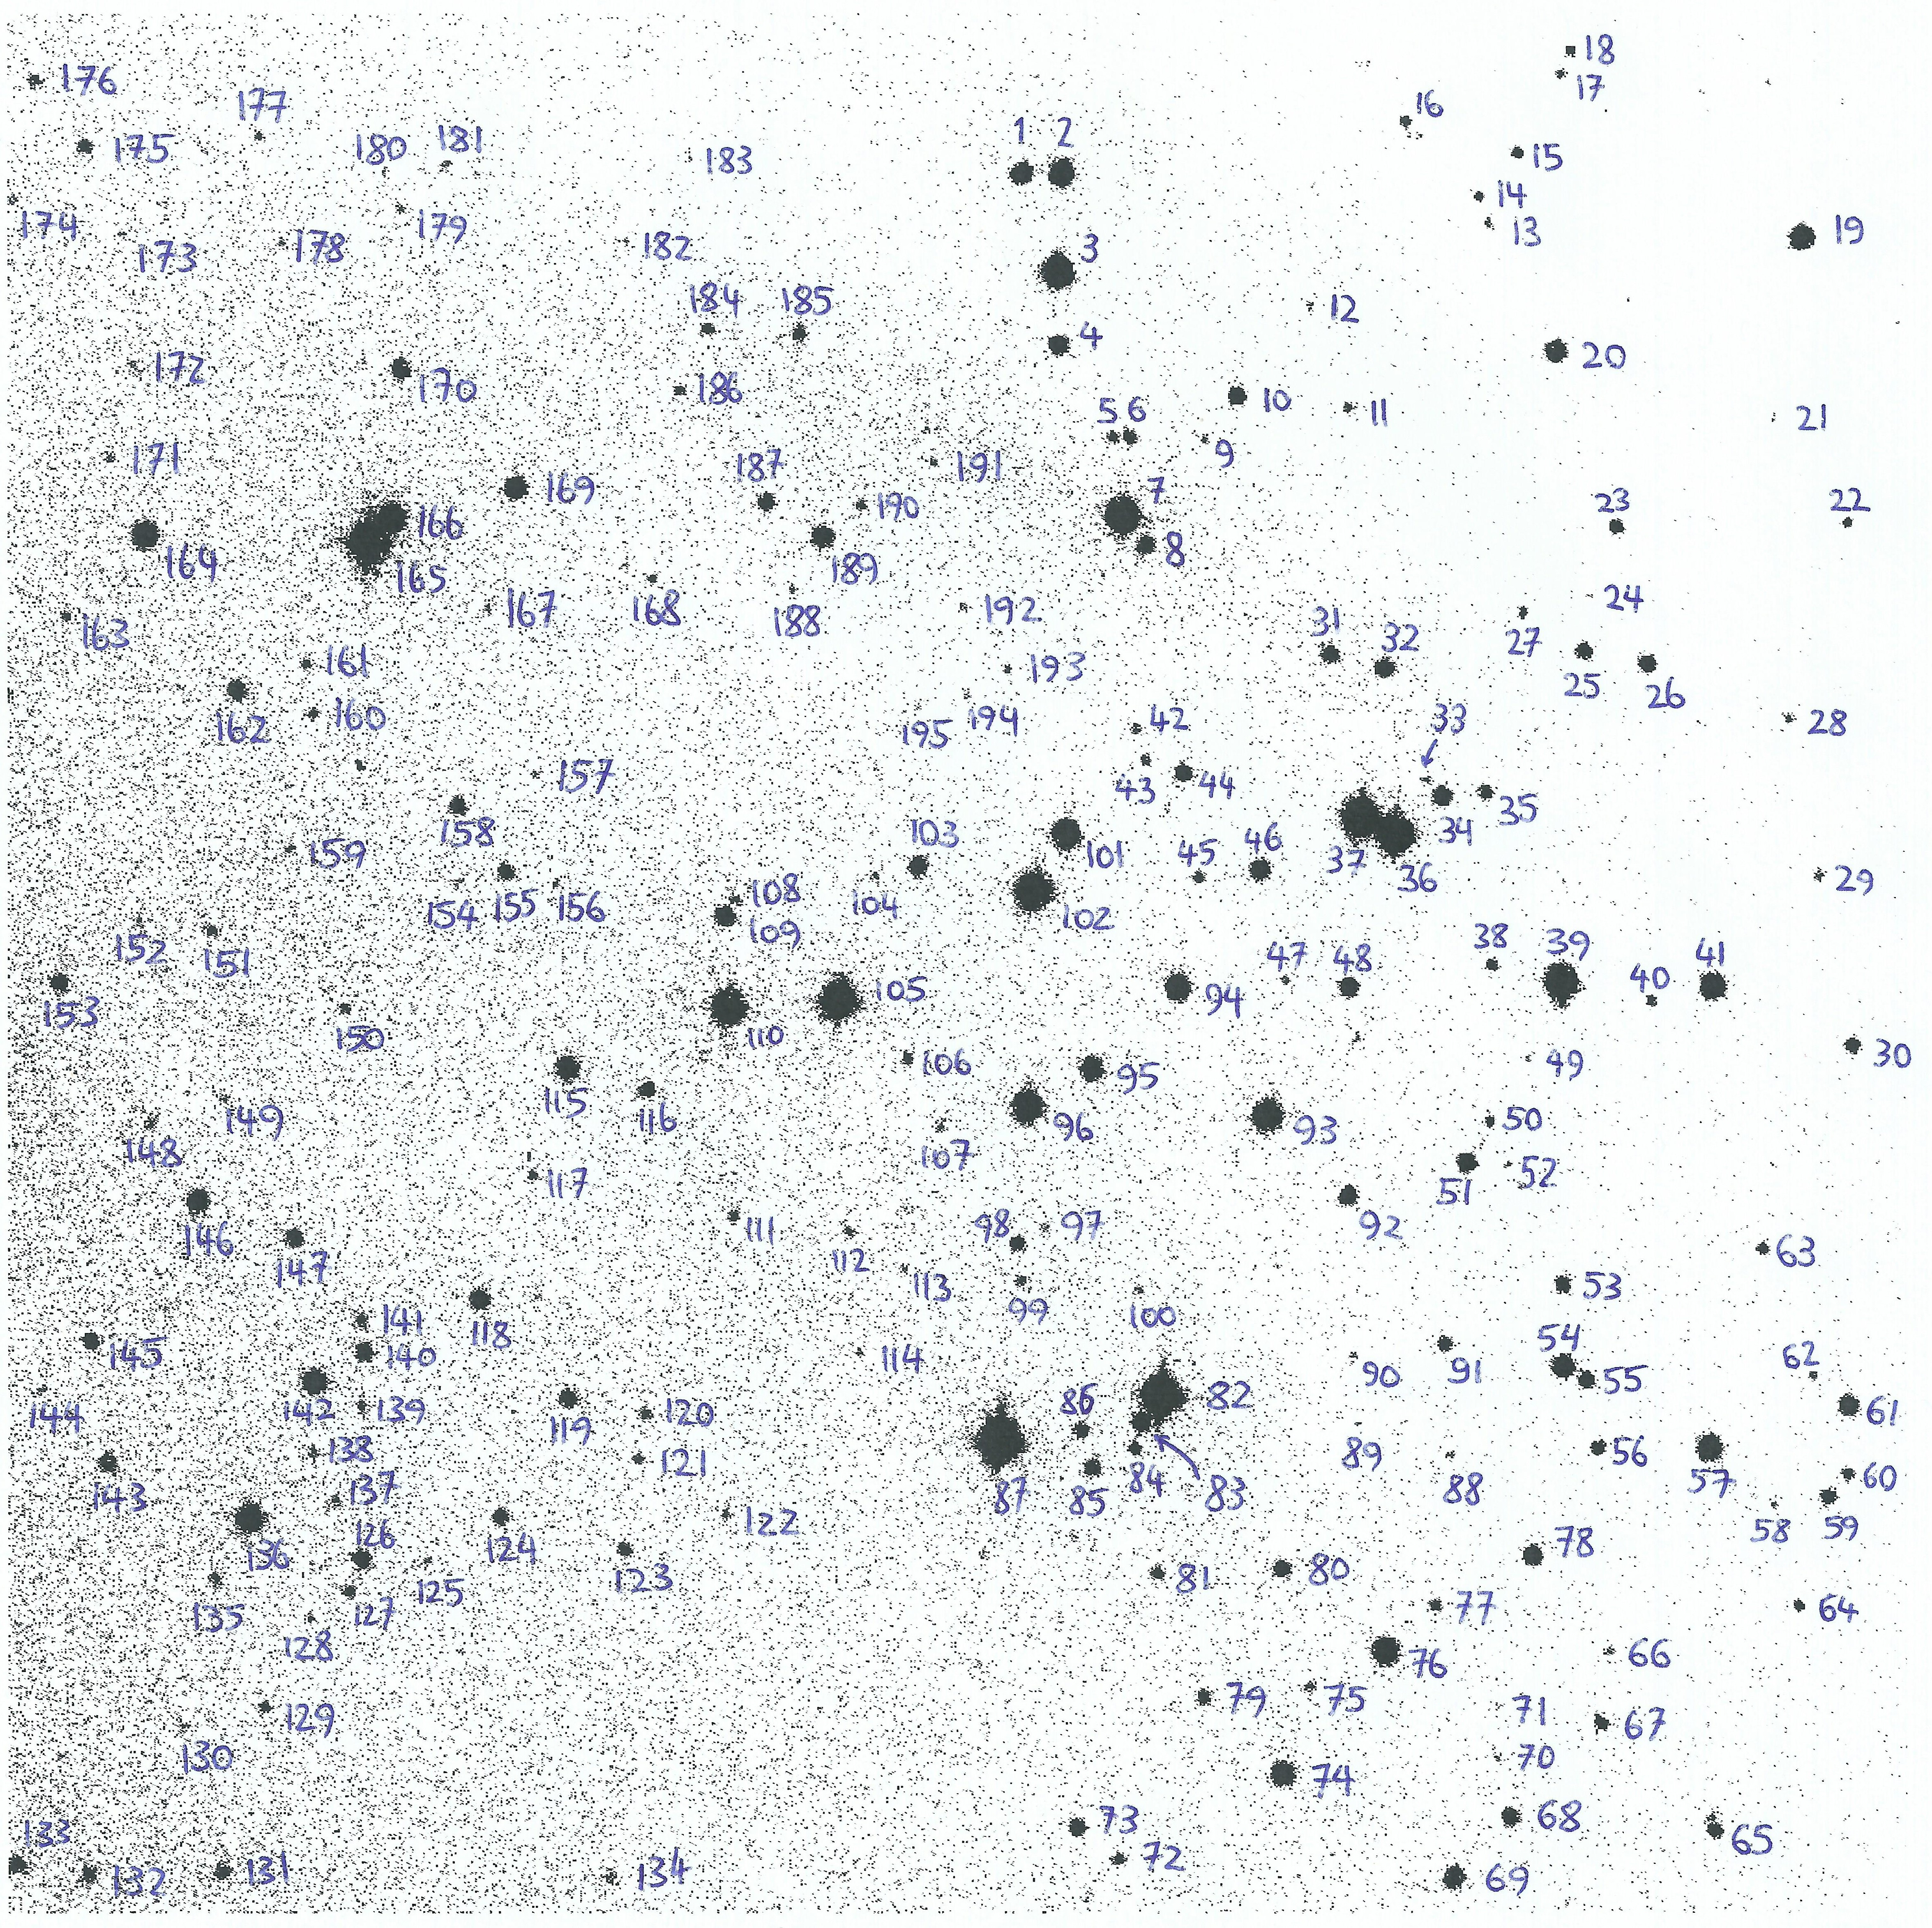
\includegraphics[width=0.95\textwidth]{obsM34_num.jpg}
  \caption{Our observation of M34 in the red filter with an exposure time of 150 seconds. The numbers are in correspondence with those in image \ref{fig:DSS2M34_num}.}
  \label{fig:obsM34_num}
\end{figure}

\begin{figure}[H]
  \centering
    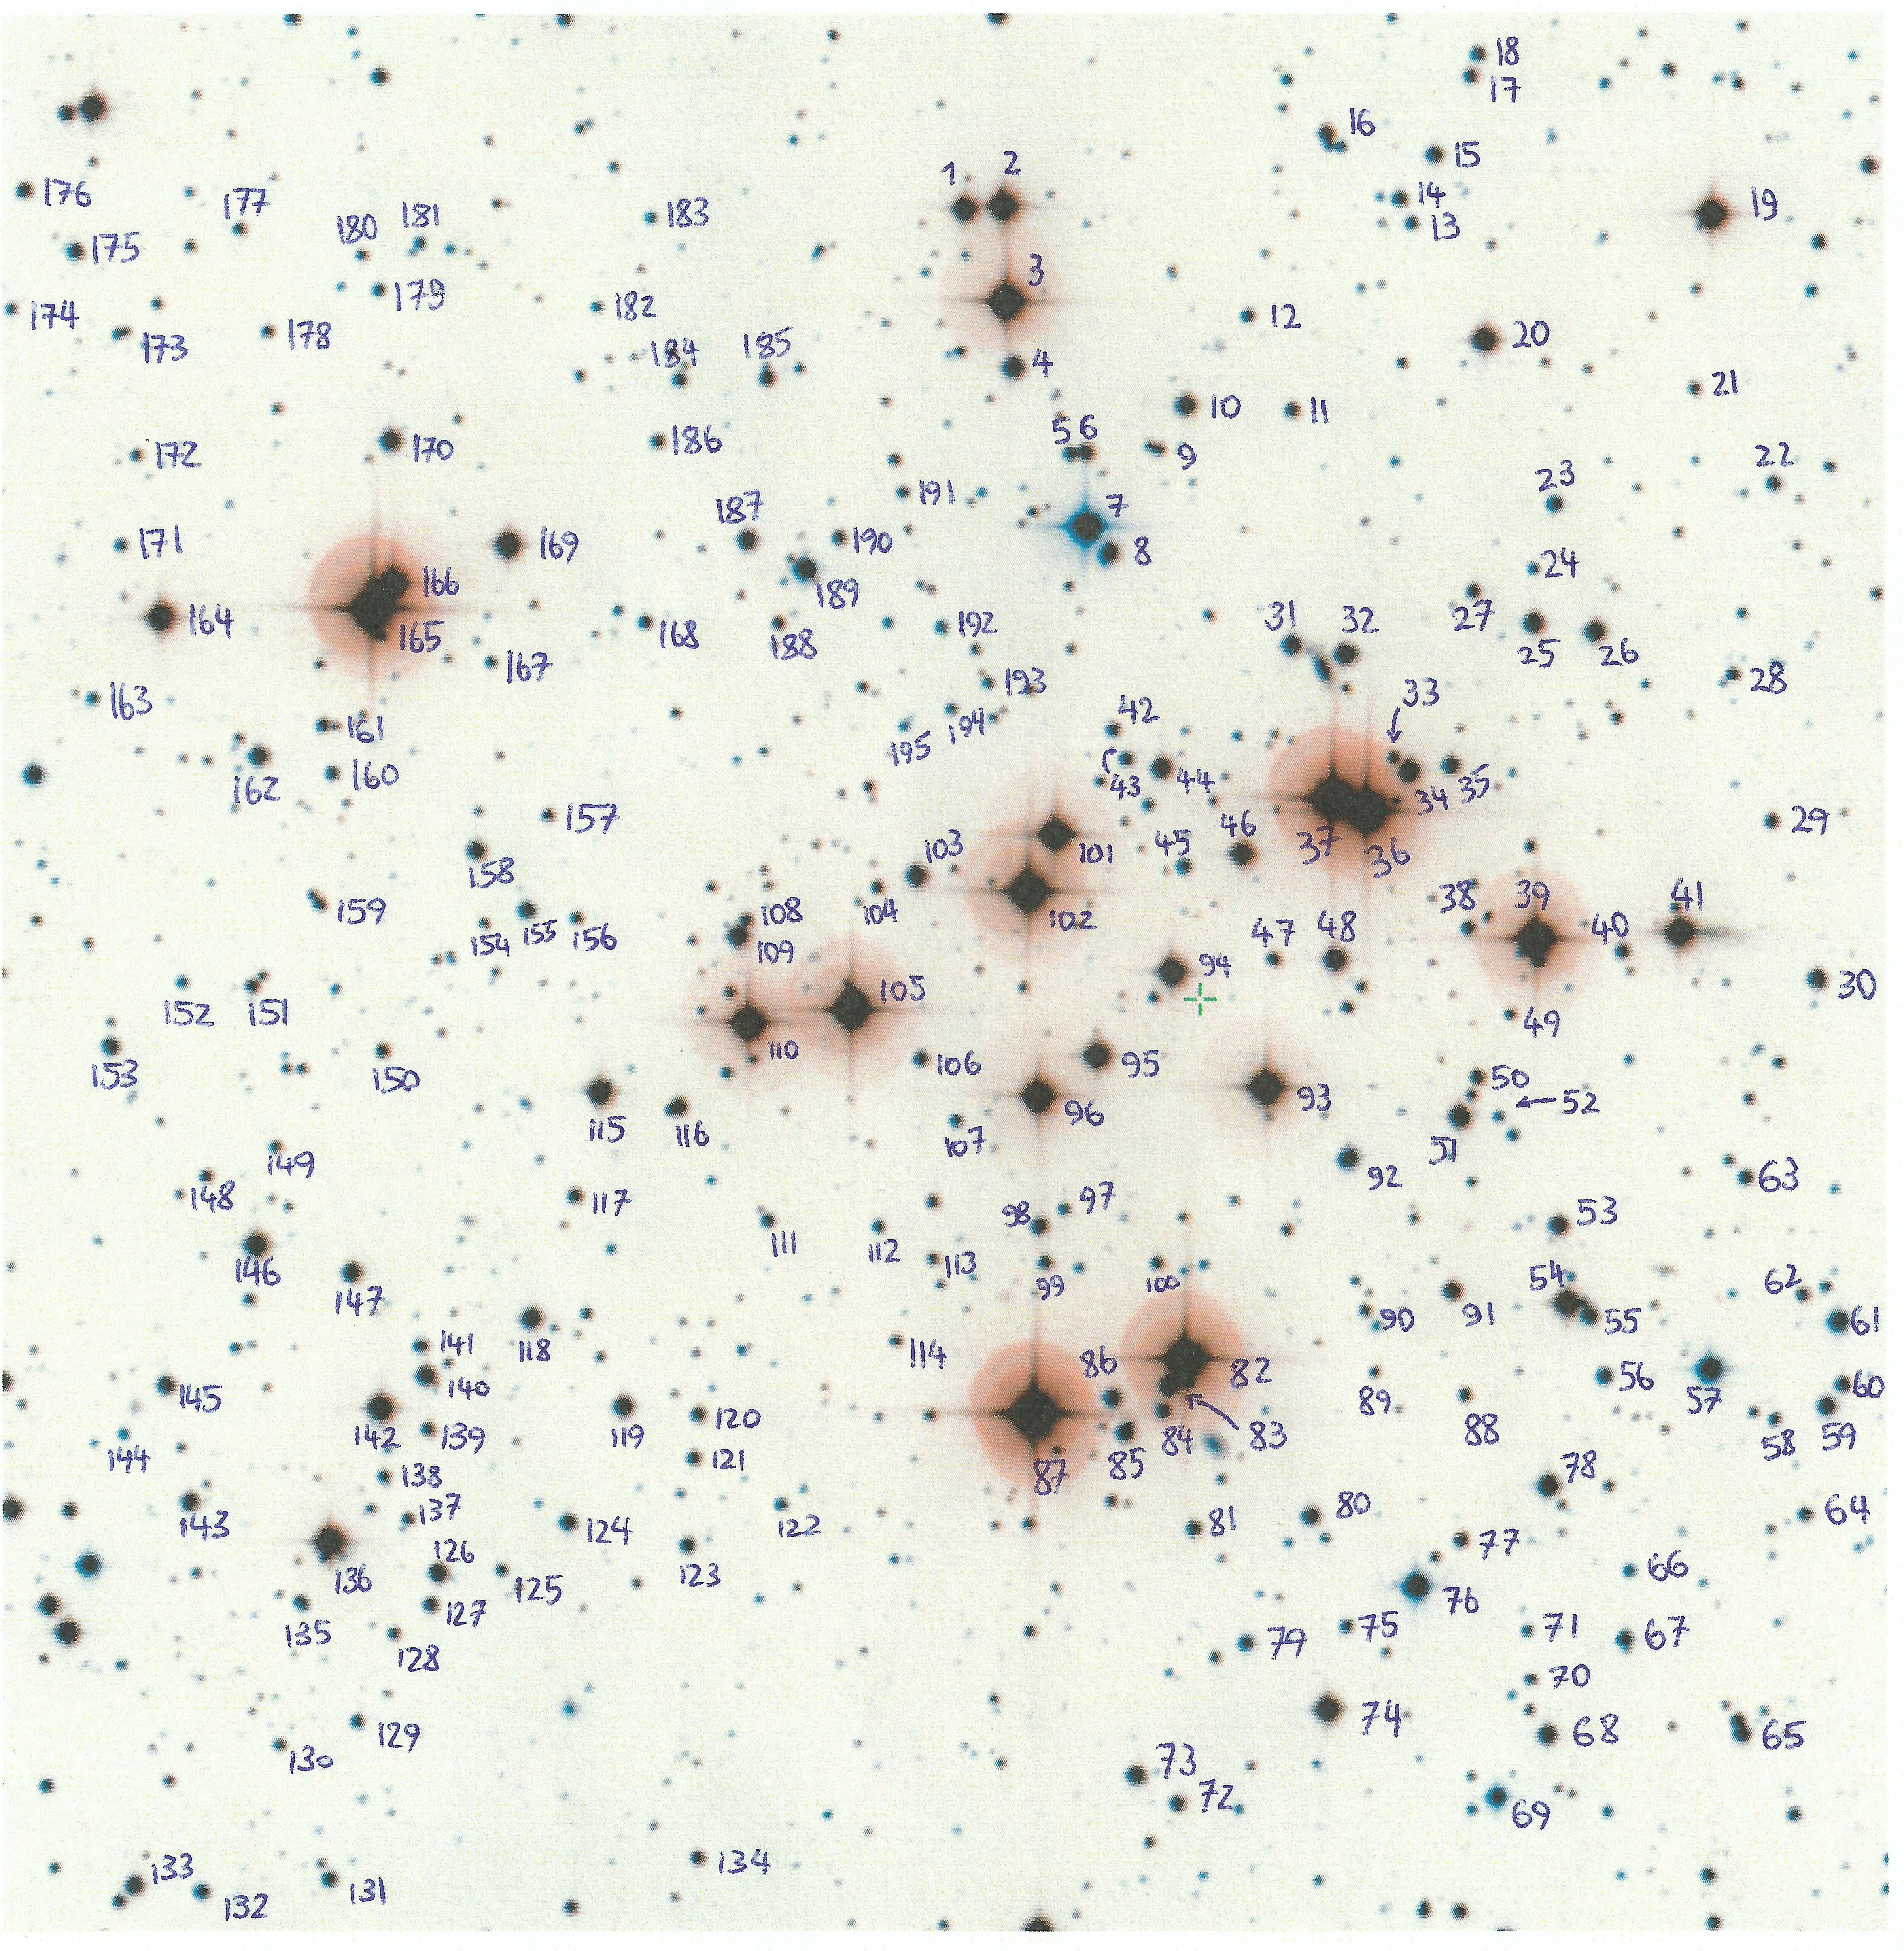
\includegraphics[width=0.95\textwidth]{DSS2M34_num.jpg}
  \caption{The negative of the observation of M34 by the DSS2. This picture was extracted from \textit{Aladin}. The numbers are in correspondence with those in image \ref{fig:obsM34_num}.}
  \label{fig:DSS2M34_num}
\end{figure}

\begin{figure}[H]
  \centering
    \includegraphics[trim={0 1.6cm 0 2.3cm},clip, width=0.95\textwidth]{M34_pm.pdf}
  \caption{Every point is an extracted source. The size corresponds to the Gaia magnitude. The arrows illustrate the direction of the proper motion. A star was for example not analysed if the proper motions were missing.}
  \label{fig:M34_pm}
\end{figure}

Figure \ref{fig:M34_pm} already illustrates that most stars are moving in the negative declination direction. One can also see some high proper motion stars.

\begin{figure}[H]
  \centering
    \includegraphics[trim={0 3.4cm 0 2.9cm},clip,width=0.95\textwidth]{M34_histogram_all.pdf}
  \caption{Histogram of the analysed stars. In order to determine the Cluster members (CMs) an iterative sigma clipping procedure was applied (see beginning of \ref{sec:CMs}). \textbf{a, c, e}: The distances and proper motions for all stars and the CMs (in gray). \textbf{b, d, f}: This zoom-in also includes a gaussian fit of the CMs. Above those plots the mean and sigma of this gaussian.}
  \label{fig:M34_histogram_all}
\end{figure}

\begin{figure}[H]
  \centering
    \includegraphics[trim={0 0 2cm 0},clip,width=0.95\textwidth]{M34_histogram_RV.pdf}
  \caption{An histogram of the radial velocities. In gray our cluster members determined with figure \ref{fig:M34_histogram_all}. We see that non of the outliers are also CMs. This is what we would expect.}
  \label{fig:M34_histogram_RV}
\end{figure}

\begin{figure}[H]
  \centering
    \includegraphics[trim={0 0.4cm 0 0.2cm},clip,width=0.65\textwidth]{M34_histogram_mags.pdf}
  \caption{The distribution of Gaia magnitudes of the analysed stars.}
  \label{fig:M34_histogram_mags}
\end{figure}

\begin{figure}[H]
  \centering
    \includegraphics[trim={0 0.5cm 0 0.5cm},clip,width=0.97\textwidth]{M34_pm_scatter_sigma.pdf}
  \caption{The proper motions of all analysed stars including the proper motion of the cluster (red) extracted in figure \ref{fig:M34_histogram_all}. The right side is a zoom-in of the left side.}
  \label{fig:M34_pm_scatter_sigma}
\end{figure}


\begin{figure}[H]
  \centering
    \includegraphics[trim={0 1.6cm 0 2.3cm},clip,width=0.95\textwidth]{M34_pm_mask.pdf}
  \caption{Similar to figure \ref{fig:M34_pm} yet just including our cluster members (CMs).}
  \label{fig:M34_pm_mask}
\end{figure}

Those last few plots clearly shows us that those stars really make us a cluster. Our cluster distance of (509 $\pm$ 26) pc agrees with the literature value of 513 pc. We want to bring up that SIMBAD incorrectly classifies some stars as member stars of M34. E.g. \textit{Gaia DR2 337177889338182400\footnote{\url{http://simbad.u-strasbg.fr/simbad/sim-basic?Ident=Gaia+DR2+337177889338182400&submit=SIMBAD+search}}} - this star has an distance of (126 $\pm$ 1) pc according to \textit{Gaia}. This would be about 400 parsec away from the core of the cluster. 

%http://simbad.u-strasbg.fr/simbad/sim-ref?bibcode=2018A%26A...618A..93C


\begin{table}[H]
\centering
\caption{All \textit{Gaia Source ID}s of our identified cluster members (CMs) of M34.}
\begin{tabular}{lllll}
337189979669777024 & 337165657269539712 & 337151604138401024 & 337176446229194752 & 337173663090374272 \\
337189640368700416 & 337154215478462720 & 337151707217611520 & 337176240070775424 & 337174006687749504 \\
337189842231829632 & 337154146758992000 & 337152153894211712 & 337176377509719424 & 337175415437021824 \\
337167370961929600 & 337154073743193088 & 337153184686353280 & 337149783072247424 & 337175346717538304 \\
337167066020594304 & 337153631361117952 & 337153322125297408 & 337149748712509440 & 337178439093990656 \\
337167169099820416 & 337165378097895424 & 337152561914712320 & 337172975895643648 & 337178503517166208 \\
337166134011354624 & 337165275017903744 & 337154112399259008 & 337172112606444672 & 337177167783677056 \\
337165584255547008 & 337153493924213888 & 337153837521355520 & 337172323060610944 & 337177236503146624 \\
337165966508978688 & 337153493923993344 & 337153837521356928 & 337173147694323968 & 337178851410839040 \\
337165829070036608 & 337163698766294784 & 337152978527902592 & 337173078974848000 & 337177545740806656 \\
337165932149250176 & 337164038067322368 & 337153081607118080 & 337172288701093632 &                    \\
337165481176331008 & 337163630046824064 & 337177408301862784 & 337173525651437568 &                    \\
337165652975852160 & 337151840360210688 & 337177373942124672 & 337173113334580224 &                   
\end{tabular}
\end{table}



\begin{table}[H]
\centering
\caption{\textit{Gaia Source ID}s of the non CMs of M34.}
\begin{tabular}{lllll}
337190014029514240 & 337177614460287360 & 337152566211055744 & 337172219981402496 & 337175552875962368 \\
337190018325811456 & 337177614460290048 & 337152944168176640 & 337171945103720832 & 337175651659849856 \\
337177850682133760 & 337154181118730752 & 337153425204519040 & 337171910743987968 & 337176033912291456 \\
337177820618702848 & 337154078039521536 & 337153356485035904 & 337171876382612992 & 337176063976748160 \\
337189571649224832 & 337165416753189760 & 337153459564251520 & 337124936685069824 & 337176068272026368 \\
337177820618707712 & 337165382393453056 & 337153974960313344 & 337149302035925248 & 337176171351238656 \\
337177717539493504 & 337152012158896256 & 337152978527905664 & 337172975895640064 & 337178679612144128 \\
337189567352918400 & 337163733124237824 & 337177404005543552 & 337173078974851584 & 337178640957119744 \\
337189743447917696 & 337163698766295808 & 337176618028304128 & 337173078974849664 & 337178847115567360 \\
337190568081631488 & 337163698766295936 & 337176583668152448 & 337172662361656320 & 337178920130314112 \\
337190568081630464 & 337164003707585920 & 337153115966851328 & 337173525651433344 & 337179538605845248 \\
337190563785327232 & 337164008003935744 & 337176652387618432 & 337173525651432832 & 337179607325083520 \\
337190666871477760 & 337151913376040704 & 337176648091300736 & 337173800529335680 & 337178026777124736 \\
337190632505871744 & 337151810296828288 & 337152841089175168 & 337173697450114176 & 337178091200302592 \\
337190636801101312 & 337151638498142464 & 337153012887641600 & 337172907176365824 & 337178022481798912 \\
337167203459553280 & 337151702921857536 & 337152806729441664 & 337176824184478080 & 337177923697917696 \\
337167031660864640 & 337152119534475136 & 337176377509721088 & 337176789826567424 & 337177889338184576 \\
337166172667408512 & 337152394412380032 & 337173422572224768 & 337176785531080576 & 337177889338182400 \\
337166172667412096 & 337153150326620928 & 337173353852753280 & 337176892905777536 & 337177958057657344 \\
337166207027147136 & 337153146030266752 & 337173216413805312 & 337176824186301440 & 337178159920736128 \\
337166516264801920 & 337153219046094464 & 337149817431979264 & 337173903608540800 & 337177541445409664 \\
337166378825857664 & 337151943439422208 & 337149817431981568 & 337174006687747968 & 337177545740805504 \\
337165897789510528 & 337152424475762432 & 337173005959042432 & 337175552875965824 & 337177472725904512 \\
337165893493188096 & 337152531851323776 & 337172941535906432 & 337176995984984960 &                    \\
337165897789512064 & 337152566211055104 & 337172219981401856 & 337178537876901888 &                   
\end{tabular}
\end{table}






\paragraph{Teutsch 55}

\begin{figure}[H]
  \centering
    \includegraphics[width=0.95\textwidth]{obsTeutsch55_num.jpg}
  \caption{Our observation of Teutsch 55 in the red filter with an exposure time of 300 seconds. The numbers are in correspondence with those in image \ref{fig:DSS2Teutsch55_num}.}
  \label{fig:obsTeutsch55_num}
\end{figure}

\begin{figure}[H]
  \centering
    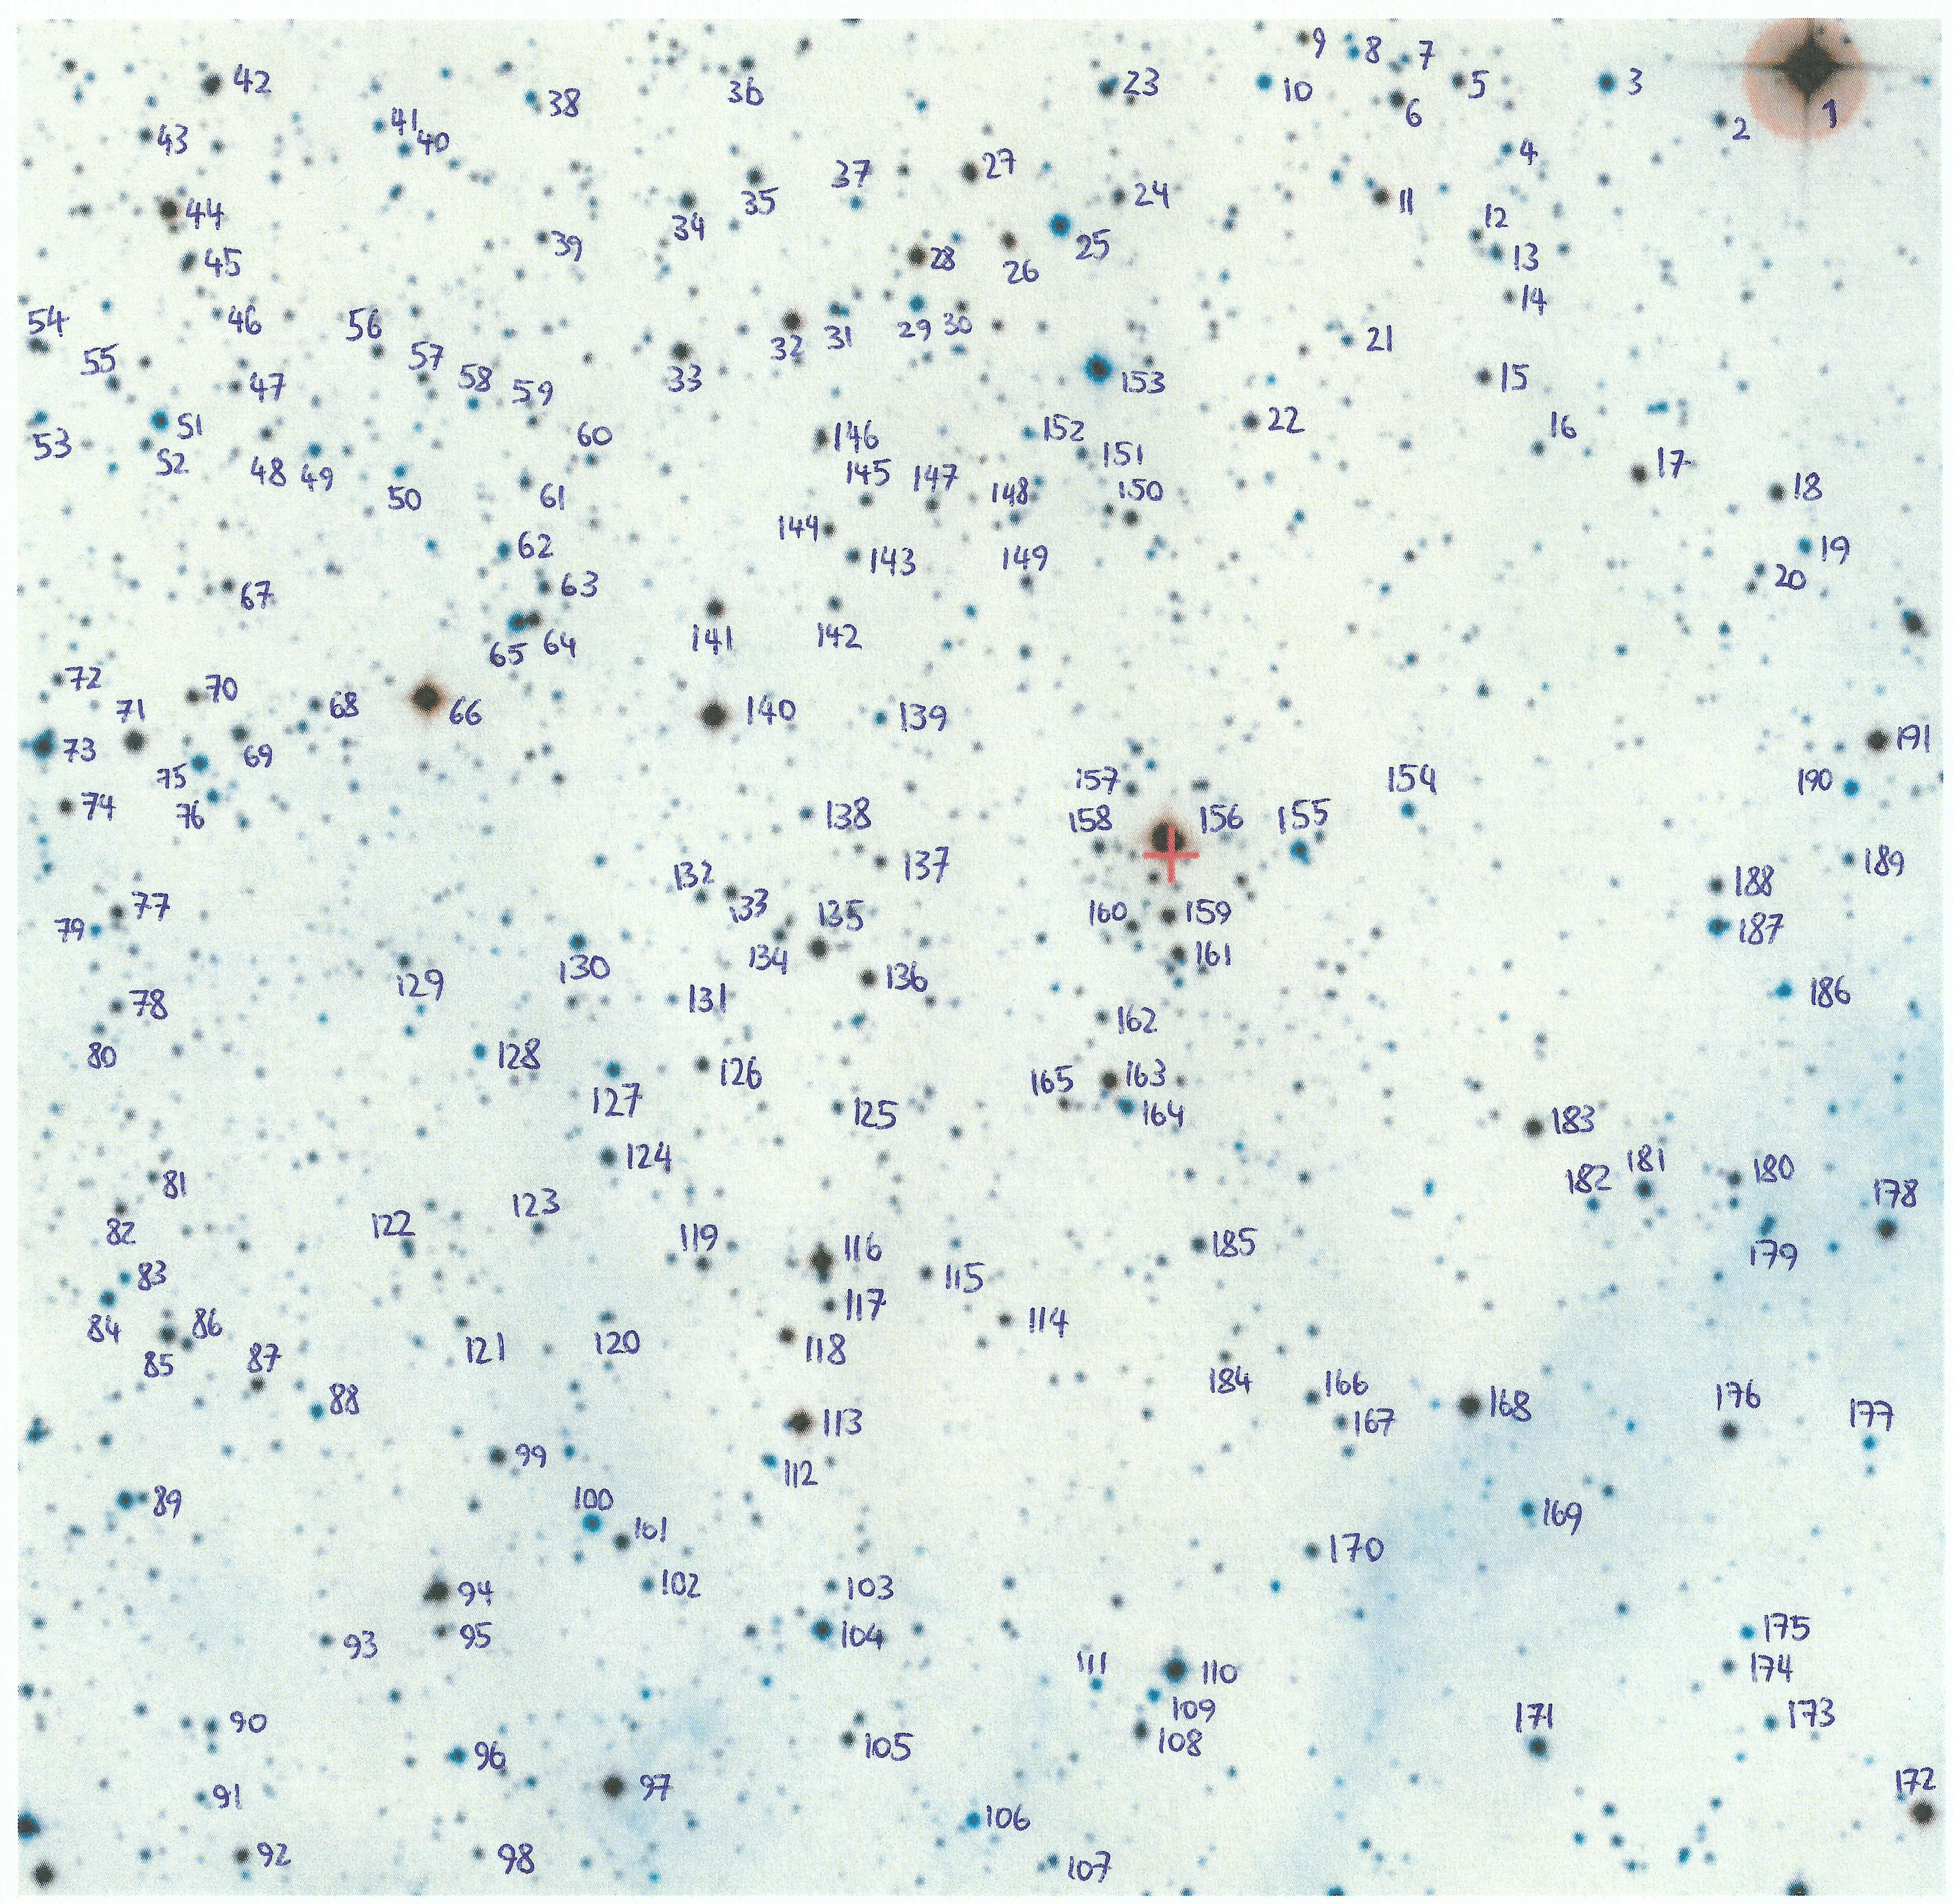
\includegraphics[width=0.95\textwidth]{DSS2Teutsch55_num.jpg}
  \caption{The negative of the observation of Teutsch 55 by the DSS2. This picture was extracted from \textit{Aladin}. The numbers are in correspondence with those in image \ref{fig:obsTeutsch55_num}.}
  \label{fig:DSS2Teutsch55_num}
\end{figure}


\begin{figure}[H]
  \centering
    \includegraphics[trim={0 1.6cm 0 2.3cm},clip, width=0.95\textwidth]{Teutsch55_pm.pdf}
  \caption{Every point is an extracted source. The size corresponds to the Gaia magnitude. The arrows illustrate the direction of the proper motion. A star was for example not analysed if the proper motions were missing.}
  \label{fig:Teutsch55_pm}
\end{figure}

Notice the high proper motion stars in figure \ref{fig:Teutsch55_pm}. 

\begin{figure}[H]
  \centering
    \includegraphics[trim={0 3.4cm 0 2.9cm},clip,width=0.95\textwidth]{Teutsch55_histogram_all.pdf}
  \caption{Histogram of the analysed stars. In order to determine the Cluster members (CMs) an iterative sigma clipping procedure was applied (see beginning of \ref{sec:CMs}). \textbf{a, c, e}: The distances and proper motions for all stars and the CMs (in gray). \textbf{b, d, f}: This zoom-in also includes a gaussian fit of the CMs. Above those plots the mean and sigma of this gaussian.}
  \label{fig:Teutsch55_histogram_all}
\end{figure}

\begin{figure}[H]
  \centering
    \includegraphics[trim={0 0 2cm 0},clip,width=0.95\textwidth]{Teutsch55_histogram_RV.pdf}
  \caption{An histogram of the radial velocities. In gray our cluster members determined with figure \ref{fig:Teutsch55_histogram_all}. We see that non of the outliers are also CMs. This is what we would expect.}
  \label{fig:Teutsch55_histogram_RV}
\end{figure}

\begin{figure}[H]
  \centering
    \includegraphics[trim={0 0.4cm 0 0.2cm},clip,width=0.65\textwidth]{Teutsch55_histogram_mags.pdf}
  \caption{The distribution of Gaia magnitudes of the analysed stars.}
  \label{fig:Teutsch55_histogram_mags}
\end{figure}

\begin{figure}[H]
  \centering
    \includegraphics[trim={0 0.5cm 0 0.5cm},clip,width=0.97\textwidth]{Teutsch55_pm_scatter_sigma.pdf}
  \caption{The proper motions of all analysed stars including the proper motion of the cluster (red) extracted in figure \ref{fig:Teutsch55_histogram_all}. The right side is a zoom-in of the left side.}
  \label{fig:Teutsch55_pm_scatter_sigma}
\end{figure}


\begin{figure}[H]
  \centering
    \includegraphics[trim={0 1.6cm 0 2.3cm},clip,width=0.95\textwidth]{Teutsch55_pm_mask.pdf}
  \caption{Similar to figure \ref{fig:Teutsch55_pm} yet just including our cluster members (CMs).}
  \label{fig:Teutsch55_pm_mask}
\end{figure}

In contrast to figure \ref{fig:M34_pm_mask} we do not see, that those stars are moving as a group in one direction. We also see this very broad distribution in distances and proper motions in figure \ref{fig:Teutsch55_histogram_all}. So we cannot really confirm this cluster.



\begin{table}[H]
\centering
\caption{All \textit{Gaia Source ID}s of our identified cluster members (CMs) of Teutsch 55.}
\begin{tabular}{lllll}
513620643419170048 & 513991522438846080 & 513603356171236864 & 513603188672284544 & 513616039214263808 \\
513620471620472576 & 513991041402525952 & 513602604556727168 & 513603257391604352 & 513614561745676160 \\
513620402900999680 & 513991007042793856 & 513602604556729856 & 513615145861079808 & 513614561745520896 \\
513620505980209280 & 513979320431655168 & 513602600256983168 & 513614974062383360 & 513614527385939584 \\
513620162382821376 & 513979324731745408 & 513602570196995840 & 513615008422120832 & 513614458666310784 \\
513620093663346560 & 513979702688856704 & 513602192239875712 & 513603704068348800 & 513614458666314624 \\
513619750065972608 & 513979324731738624 & 513602913794383360 & 513615042781850112 & 513614458666316800 \\
513619646986761600 & 513991213200956800 & 513602119220208384 & 513615077141594880 & 513613702752071168 \\
513619612627027200 & 513991208901147648 & 513601745563300096 & 513615317659755776 & 513613908910524288 \\
513618100798551680 & 513991178841219200 & 513602020441196416 & 513615283300017536 & 513613904611707648 \\
513618822353389184 & 513615867415543552 & 513602776355441024 & 513615283300021760 & 513613049917218560 \\
513618719273849216 & 513615867415546624 & 513600508612716032 & 513615180220811264 & 513607655438172544 \\
513619372108862720 & 513615833055812864 & 513600508612723200 & 513615248940279936 & 513607999035549056 \\
513619887504920576 & 513615622598206336 & 513601367606164864 & 513616107933729664 & 513608033395284480 \\
513619814486284416 & 513615558173884544 & 513601573764596096 & 513615798696076544 & 513608033395282304 \\
513616898207875200 & 513979187292805760 & 513601539400829568 & 513616520250583680 & 513608205193962752 \\
513616898207683584 & 513603841507296768 & 513601505044977920 & 513616588970057344 & 513611052753420160 \\
513616829488210688 & 513979152933080192 & 513601466386006016 & 513616520250578944 & 513617134427177216 \\
513616898207688576 & 513979084213598720 & 513601058368394752 & 513616588970054272 & 513614149428684288 \\
513616932567425024 & 513979084213601792 & 513612706319704320 & 513616623329788928 & 513614252507894016 \\
513616726408994944 & 513979015494118784 & 513612775039173760 & 513616588970055552 & 513613938971458176 \\
513616966927154560 & 513978912414908416 & 513612878118387456 & 513616417171365632 & 513614321227373184 \\
513992278352841600 & 513978912414914560 & 513613359154704128 & 513616382811631488 & 513617379244080640 \\
513616928269018368 & 513979084213604992 & 513613530953392896 & 513616451531105920 & 513617482323287552 \\
513992140913887360 & 513603772787821056 & 513613427874173440 & 513616485890839552 & 513617447963853184 \\
513992037834676096 & 513603566629392128 & 513613457934694272 & 513619440828334464 & 513618306957312512 \\
513991419359381376 & 513603497909917952 & 513613462233912576 & 513617654121970176 & 513618306957002368 \\
513991762957004416 & 513603497909915776 & 513613393514437120 & 513614802263686912 &                    \\
513991556798575616 & 513603497909918720 & 513602982513857024 & 513616245372852736 &                   
\end{tabular}
\end{table}



\begin{table}[H]
\centering
\caption{\textit{Gaia Source ID}s of the non CMs of Teutsch 55.}
\begin{tabular}{lllll}
513619234669893120 & 513619917573669120 & 513615936135015552 & 513612981197602688 & 513616485890837504 \\
513619784425703936 & 513616996987737216 & 513615936135019776 & 513601608124185216 & 513613870251555328 \\
513620540339946112 & 513616692049256832 & 513615833055811072 & 513614870983181696 & 513607964675796864 \\
513619784425700992 & 513992067894589056 & 513602565896806656 & 513603119952661248 & 513607861596594176 \\
513619646986763264 & 513991384999644672 & 513601745563294976 & 513603016873591936 & 513611435009360000 \\
513619612627031680 & 513991075762257792 & 513602772055238016 & 513603291751491072 &                    \\
513618135158287360 & 513991041402529664 & 513601157147534976 & 513615175921610752 &                    \\
513618787993324288 & 513990972682789376 & 513602840774713984 & 513615352019490432 &                    \\
513619578267289216 & 513979633969386368 & 513612775039175808 & 513615764332333184 &                   
\end{tabular}
\end{table}




\paragraph{Stock 19 (C0001+557)}

\begin{figure}[H]
  \centering
    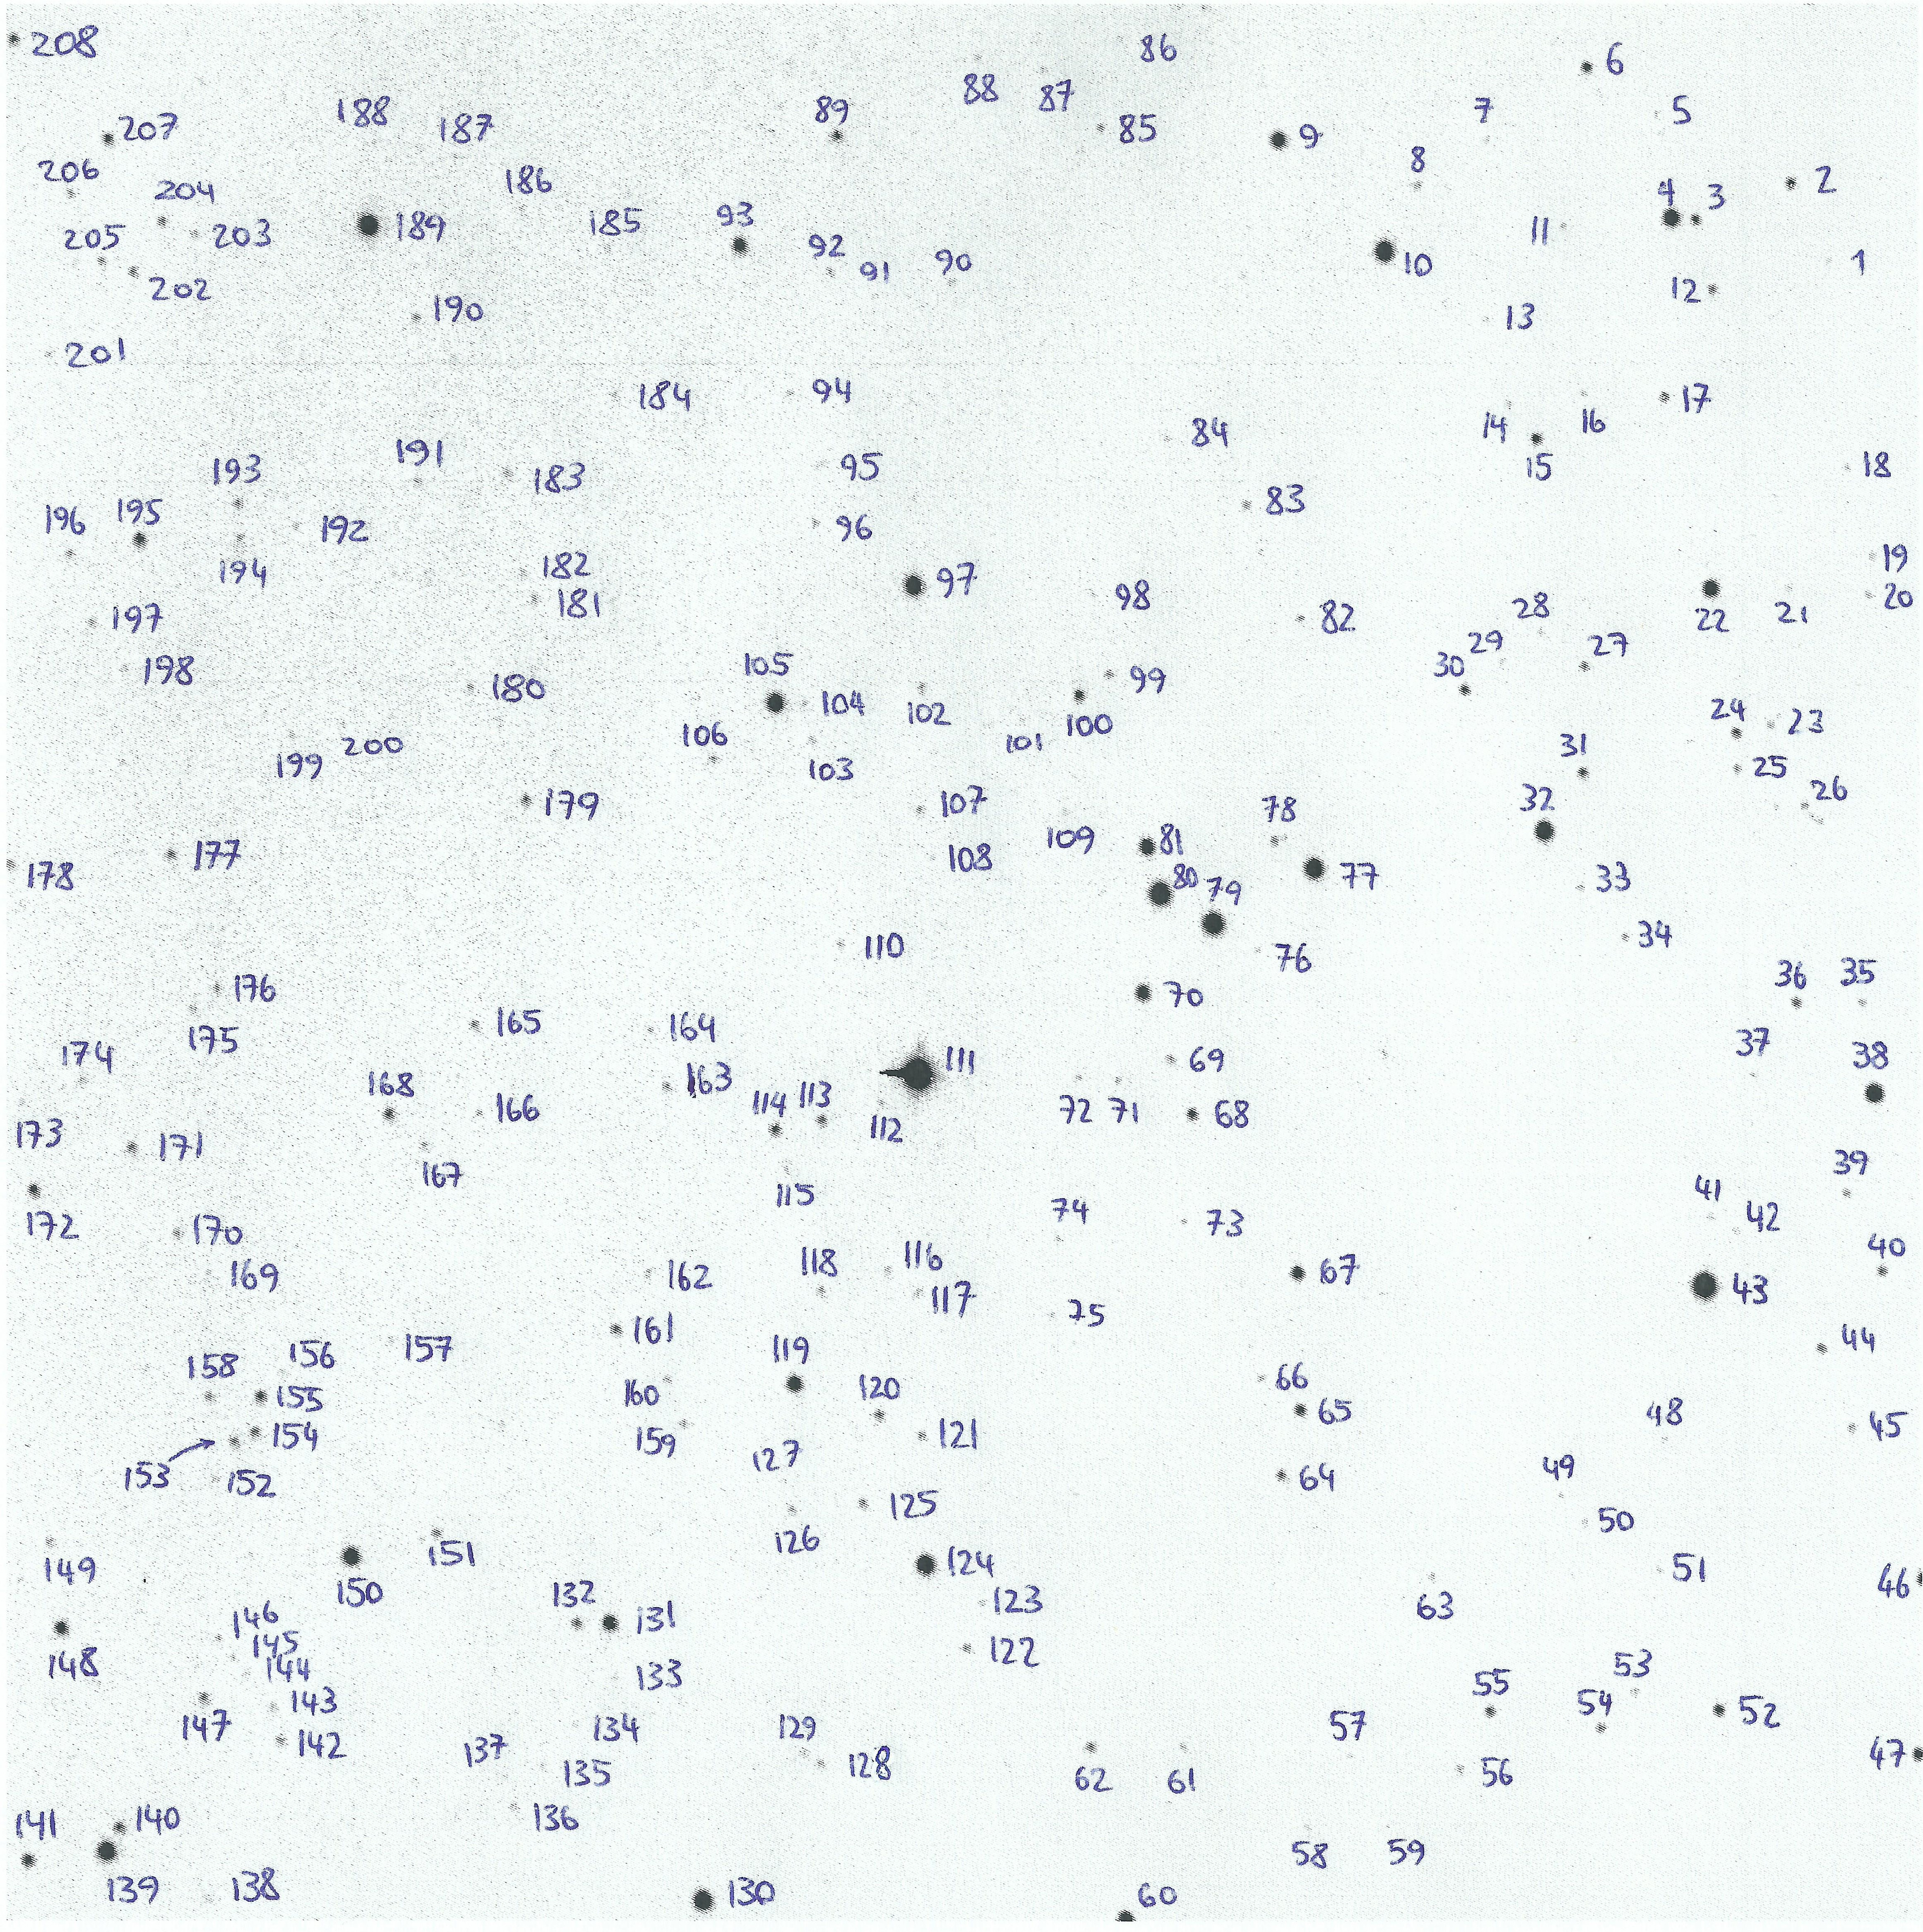
\includegraphics[width=0.95\textwidth]{obsStock19_num.jpg}
  \caption{Our observation of Stock 19 in the red filter with an exposure time of 200 seconds. The numbers are in correspondence with those in image \ref{fig:DSS2Stock19_num}.}
  \label{fig:obsStock19_num}
\end{figure}

\begin{figure}[H]
  \centering
    \includegraphics[width=0.95\textwidth]{DSS2Stock19_num.jpg}
  \caption{The negative of the observation of Stock 19 by the DSS2. This picture was extracted from \textit{Aladin}. The numbers are in correspondence with those in image \ref{fig:obsStock19_num}.}
  \label{fig:DSS2Stock19_num}
\end{figure}

The only light source we observed - of the about 600 - without a Gaia DR2 entry is star 124 (in the lower middle of \ref{fig:obsStock19_num} and \ref{fig:DSS2Stock19_num}) known as TYC 3656-465-1. 


\begin{figure}[H]
  \centering
    \includegraphics[trim={0 1.6cm 0 2.3cm},clip, width=0.95\textwidth]{Stock19_pm.pdf}
  \caption{Every point is an extracted source. The size corresponds to the Gaia magnitude. The arrows illustrate the direction of the proper motion. A star was for example not analysed if the proper motions were missing.}
  \label{fig:Stock19_pm}
\end{figure}

In contrast to figure \ref{fig:M34_pm}, a prefered direction of the stars we observed is not directly apparent. 


\begin{figure}[H]
  \centering
    \includegraphics[trim={0 3.4cm 0 2.9cm},clip,width=0.95\textwidth]{Stock19_histogram_all.pdf}
  \caption{Histogram of the analysed stars. In order to determine the Cluster members (CMs) an iterative sigma clipping procedure was applied (see beginning of \ref{sec:CMs}). \textbf{a, c, e}: The distances and proper motions for all stars and the CMs (in gray). \textbf{b, d, f}: This zoom-in also includes a gaussian fit of the CMs. Above those plots the mean and sigma of this gaussian.}
  \label{fig:Stock19_histogram_all}
\end{figure}

\begin{figure}[H]
  \centering
    \includegraphics[trim={0 0 2cm 0},clip,width=0.95\textwidth]{Stock19_histogram_RV.pdf}
  \caption{An histogram of the radial velocities. In gray our cluster members determined with figure \ref{fig:Stock19_histogram_all}.}
  \label{fig:Stock19_histogram_RV}
\end{figure}

\begin{figure}[H]
  \centering
    \includegraphics[trim={0 0.4cm 0 0.2cm},clip,width=0.65\textwidth]{Stock19_histogram_mags.pdf}
  \caption{The distribution of Gaia magnitudes of the analysed stars.}
  \label{fig:Stock19_histogram_mags}
\end{figure}

\begin{figure}[H]
  \centering
    \includegraphics[trim={0 0.5cm 0 0.5cm},clip,width=0.97\textwidth]{Stock19_pm_scatter_sigma.pdf}
  \caption{The proper motions of all analysed stars including the proper motion of the cluster (red) extracted in figure \ref{fig:Stock19_histogram_all}. The right side is a zoom-in of the left side.}
  \label{fig:Stock19_pm_scatter_sigma}
\end{figure}


\begin{figure}[H]
  \centering
    \includegraphics[trim={0 1.6cm 0 2.3cm},clip,width=0.95\textwidth]{Stock19_pm_mask.pdf}
  \caption{Similar to figure \ref{fig:Stock19_pm} yet just including our cluster members (CMs).}
  \label{fig:Stock19_pm_mask}
\end{figure}

Similar to \ref{fig:Teutsch55_pm_mask}, but in contrast to figure \ref{fig:M34_pm_mask} we do not see, that those stars are moving as a group in one direction. We also see this very broad distribution in distances and proper motions in figure \ref{fig:Stock19_histogram_all}. So we cannot really confirm this cluster.




\begin{table}[H]
\centering
\caption{All \textit{Gaia Source ID}s of our identified cluster members (CMs) of Stock 19.}
\begin{tabular}{lllll}
420874776035616512 & 420866220460820480 & 420964970347766400 & 420862131652010752 & 420869072319131008 \\
420875188352476160 & 420866014302391680 & 420964901628291584 & 420868007167254656 & 420869415916515968 \\
420875016553783936 & 420865876863445504 & 420964901628292608 & 420867972807519616 & 420869450276248320 \\
420875050913525376 & 420865979942662016 & 420964935988030848 & 420867972807524096 & 420869450276244992 \\
420874290700505600 & 420865773784235392 & 420964759890587648 & 420867801008840960 & 420869518995713408 \\
420874294999283584 & 420865739424500096 & 420964798549079552 & 420867801008838272 & 420869725154141056 \\
420874947834311168 & 420865705064765696 & 420870962104679296 & 420867079454351232 & 420869656434657024 \\
420874810395357440 & 420864983510262784 & 420870962104682112 & 420866903351769600 & 420870549787844096 \\
420874913474575232 & 420864983510269568 & 420873882682440960 & 420867285612779520 & 420869931312547712 \\
420874501157717504 & 420865700763485696 & 420873504725321856 & 420867212591948544 & 420964523671177088 \\
420874569877191040 & 420864708632374784 & 420873436005849344 & 420867487469889280 & 420964523671176960 \\
420874707316144256 & 420865327107652352 & 420870859025472768 & 420867491771196544 & 420964558030914304 \\
420873195487658496 & 420865120949224704 & 420870790306001280 & 420867526130932864 & 420964725531434624 \\
420873195487659648 & 420866151741352704 & 420870790305998976 & 420867526130932096 & 420964695469863552 \\
420873161128172160 & 420871408781519232 & 420870824658830336 & 420867526130937472 & 420965107786724096 \\
420873023688973184 & 420871541916442880 & 420870790306005504 & 420867418747843072 & 420964454951694592 \\
420873019387938560 & 420871924177379072 & 420870446708618752 & 420868866160725888 & 420964386232348928 \\
420873023688975360 & 420871718018945024 & 420870446708621696 & 420867594843854208 & 420964386232219648 \\
420874363718770048 & 420871821098157696 & 420873294265833856 & 420869141038619136 & 420963836476410112 \\
420874363718771840 & 420871718019163904 & 420870343629413376 & 420867663569868288 & 420963664677718528 \\
420874363718773632 & 420871821098164608 & 420868831800928640 & 420869141038616448 & 420963973915527168 \\
420872920609763200 & 420871511860522624 & 420868831800930560 & 420869141038614016 & 420963595958408448 \\
420872748811076224 & 420871305702102144 & 420868831800933632 & 420869209758084992 & 420963699037458048 \\
420872778869755776 & 420872027256582656 & 420868763081458816 & 420869141038617344 & 420964111354467584 \\
420872783170817280 & 420872130335792256 & 420868694361987968 & 420868591282790016 & 420964145714196992 \\
420872538350177664 & 420872061616314752 & 420868660002250368 & 420868522563308928 & 420964214433667456 \\
420872542652648320 & 420872061616320384 & 420868694361991168 & 420868556923042304 & 420964214433667712 \\
420872473933176192 & 420871855457889792 & 420868282045138432 & 420870068751517184 & 420964145714334464 \\
420866632777656704 & 420873676524006400 & 420871236982638336 & 420870167529611392 & 420965623182941824 \\
420866594115318400 & 420874088840863616 & 420871065183955840 & 420870137470996224 & 420965623182937344 \\
420866564058188672 & 420873917042170496 & 420868213325668480 & 420870103111263488 & 420954009591365248 \\
420866495338712576 & 420967856565786112 & 420862234731211264 & 420869347197023616 &                    \\
420866220460819072 & 420967959645000448 & 420868105945182336 & 420869278477562624 &                   
\end{tabular}
\end{table}




\begin{table}[H]
\centering
\caption{\textit{Gaia Source ID}s of the non CMs of Stock 55.}
\begin{tabular}{lllll}
420874982194047872 & 420872508292912512 & 420871683659218688 & 420871065183959936 & 420869347197022720 \\
420874982194048128 & 420866564058185344 & 420873328622834432 & 420868247685405824 & 420869484635986048 \\
420875080974492416 & 420866564058185728 & 420968028364475008 & 420868007167253376 & 420963424159736192 \\
420968097083952384 & 420866460978978944 & 420965039067239680 & 420867869728312704 & 420964317512743808 \\
420874535517455232 & 420912880987436672 & 420870893385206016 & 420867526130931072 & 420963905195885824 \\
420874604236930816 & 420866426619243648 & 420873436005847168 & 420868350764636544 & 420963664677718656 \\
420873058048713984 & 420865533266258560 & 420868763081461376 & 420867659268629504 & 420963664677878784 \\
420872954969497600 & 420871374421576320 & 420868586978944768 & 420868419484095360 & 420963630318149504
\end{tabular}
\end{table}




%S.Zieba

\newpage



\section{References}
%TODO redo refernces using biber/biblatex using authoryear style!


% References in .bib datei auslagern?!
%All of the referenced links below were accessible on \today.\\
%\begin{thebibliography}{1}
%\bibitem{Ref1} Shelyak Instruments Manual: \url{https://observatori.uv.es/images/stories/instrum/lhires.pdf}\\
%\bibitem{Ref2} Calibration Resource (1): %\url{http://www.spectro-aras.com/forum/viewtopic.php?f=8&t=1673}\\
%\bibitem{Ref3} Calibration Resource (2): %\url{http://www.eso.org/~cguirao/caos/datareduction/calibration_lamps/calibration_lamps.html}\\
%\bibitem{Ref4} Calibration Resource (3): %\url{http://www.ctio.noao.edu/noao/content/Reference-Spectra}\\
%\bibitem{Ref5} Littrow Configuration: %\url{https://www.zfm.tu-chemnitz.de/download/pdf/annual_report_2004/81-82.pdf}\\
%\bibitem{Ref6} IRAF notes for Observational Astrophysics I, SS Larsen (2011): %\url{www.astro.ru.nl/~slarsen/teaching/OA1UU/OA1_1112/.../iraf.pdf}\\
%\bibitem{Ref7} Kaufer et al. (1997), Long-term spectroscopic monitoring of BA-type supergiants: %III. Variability of photospheric lines
%\\\\\\\\\\\\\\\\\\\\\
%\end{thebibliography}

\end{document}

